%%%%%%%%%%%%%%%%%%%%%%%%%%%%%%%%%%%%%%%%%%%%%%%%%%%%%%%%%%%
\begin{frame}[fragile]\frametitle{Objective}

To understand

			\begin{center}
			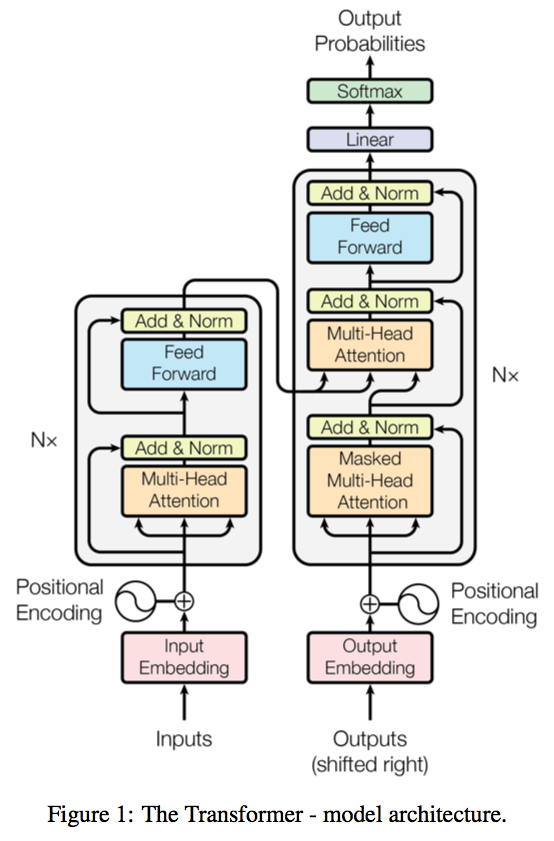
\includegraphics[width=0.35\linewidth,keepaspectratio]{transformer}
			
			{\tiny From ``Attention is all you need'' paper by Vaswani, et al., 2017}
			\end{center}		

			Thats' it \ldots
			
\end{frame}

%%%%%%%%%%%%%%%%%%%%%%%%%%%%%%%%%%%%%%%%%%%%%%%%%%%%%%%%%%%
\begin{frame}[fragile]\frametitle{Assuming Familiarity with \ldots}

\begin{itemize}
\item Linear Algebra: Vectors, Matrices
\item Calculus: Gradient Descent
\item Statistics: Distributions
\item Machine Learning: Supervised, Softmax
\item Deep Learning: Back-propagation, 
\item Natural Language Processing: Tokenization, Word Vectors, Seq2Seq (RNN, LSTM)
\end{itemize}	

\end{frame}


%%%%%%%%%%%%%%%%%%%%%%%%%%%%%%%%%%%%%%%%%%%%%%%%%%%%%%%%%%%
\begin{frame}[fragile]\frametitle{Sequence-to-Sequence (seq2seq)}

\begin{center}
See any issues with this traditional seq2seq paradigm?
\end{center}	

\end{frame}

%%%%%%%%%%%%%%%%%%%%%%%%%%%%%%%%%%%%%%%%%%%%%%%%%%%%%%%%%%%
\begin{frame}[fragile]\frametitle{Issues with recurrent models}


Linear interaction distance. O(sequence length) steps for distant word pairs to interact means:

\begin{itemize}
\item Hard to learn long-distance dependencies (because of vanishing gradient problems!)
\item Linear order of words is ``baked in''; not necessarily the  right way to think about sentences \ldots Meaning sentence structure of one language may not be correspondingly same as order in the other language.
\end{itemize}	 

\begin{center}
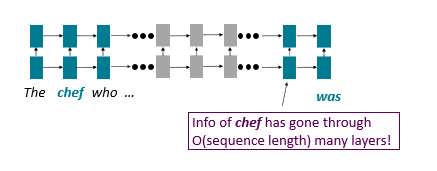
\includegraphics[width=\linewidth,keepaspectratio]{bert35}
\end{center}	

 
% {\tiny (Ref: Language \& Machine Learning - John Hewitt)}
\end{frame}

%%%%%%%%%%%%%%%%%%%%%%%%%%%%%%%%%%%%%%%%%%%%%%%%%%%%%%%%%%%
\begin{frame}[fragile]\frametitle{Issues with recurrent models}

Lack of parallelizability. Forward and backward passes have O(sequence length) unparallelizable operations

\begin{itemize}
\item GPUs can perform a bunch of independent computations at once!
\item But future RNN hidden states can’t be computed in full before past RNN
hidden states have been computed
\item Inhibits training on very large datasets!
\end{itemize}	 

\begin{center}
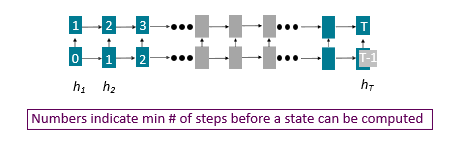
\includegraphics[width=\linewidth,keepaspectratio]{bert36}
\end{center}	

 
% {\tiny (Ref: Language \& Machine Learning - John Hewitt)}
\end{frame}

%%%%%%%%%%%%%%%%%%%%%%%%%%%%%%%%%%%%%%%%%%%%%%%%%%%%%%%%%%%
\begin{frame}[fragile]\frametitle{Then?}

If not recurrence, then what? How about word windows? Word window models aggregate local contexts

\begin{itemize}
\item Also known as 1D convolution
\item Number of unparallelizable operations not tied to sequence length!
\end{itemize}	 

\begin{center}
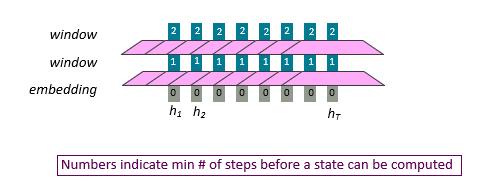
\includegraphics[width=\linewidth,keepaspectratio]{bert37}
\end{center}	

 
% {\tiny (Ref: Language \& Machine Learning - John Hewitt)}
\end{frame}

%%%%%%%%%%%%%%%%%%%%%%%%%%%%%%%%%%%%%%%%%%%%%%%%%%%%%%%%%%%
\begin{frame}[fragile]\frametitle{Then?}

What about long-distance dependencies?

\begin{itemize}
\item Stacking word window layers allows interaction between farther words
\item But if your sequences are too long, you’ll just ignore long-distance context

\end{itemize}	 

\begin{center}
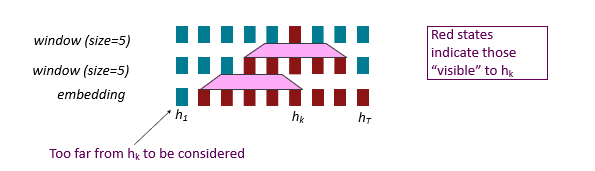
\includegraphics[width=\linewidth,keepaspectratio]{bert38}
\end{center}	

 
% {\tiny (Ref: Language \& Machine Learning - John Hewitt)}
\end{frame}

%%%%%%%%%%%%%%%%%%%%%%%%%%%%%%%%%%%%%%%%%%%%%%%%%%%%%%%%%%%
\begin{frame}[fragile]\frametitle{Attention}

If not recurrence, then what? How about attention?

\begin{itemize}
\item Attention treats each word’s representation as a query to access and  incorporate information from a set of values.
\item We saw attention from the decoder to the encoder; today we’ll think about
attention within a single sentence.
\item If attention gives us access to any state… maybe we can just use attention and don’t need the RNN?
\item Number of unparallelizable operations not tied to sequence length.
\item All words interact at every layer!

\end{itemize}	 

\begin{center}
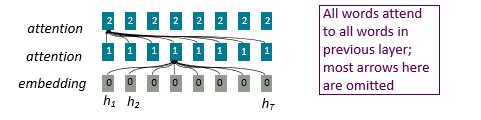
\includegraphics[width=\linewidth,keepaspectratio]{bert39}
\end{center}	

 
% {\tiny (Ref: Language \& Machine Learning - John Hewitt)}
\end{frame}

